\documentclass[pdftex,11pt]{article}
\usepackage[pdftex]{graphicx}
\usepackage{enumerate}
\usepackage{amsmath}
\usepackage{amssymb}
\usepackage{multicol}
\usepackage{algpseudocode}
\usepackage{algorithm}
\usepackage{hyperref}
\usepackage{algorithm}
\usepackage{algorithm}
\usepackage{geometry}
\usepackage{float}
\geometry{verbose,tmargin=1in,bmargin=1in,lmargin=1in,rmargin=1in}
\begin{document}
\title{COMP 540 - Homework 2}
\author{Xiang Zhou (xz58) and Guangyuan Yu (gy12)}
\title{COMP 540 Statistical Machine Learning HW2}
\maketitle
\newcommand{\pr}{\mathbb{P}}
\section{Gradient and Hessian of $NLL(\theta)$ for logistic regression}
	
	\subsection{}
	\begin{itemize}
	\item
	Given $g(z) = \frac{1}{1 + e^{-z}}$
	\begin{align*}
		\frac{\partial g(z)}{\partial z} &=-1\cdot\frac{1}{(1 + e^{-z})^{2}}\cdot-(e^{-z})\\
						&=\frac{1}{1+e^{-z}}\cdot\frac{1+e^{-z}-1}{1+e^{-z}}\\
						&=g(z)\cdot(1 - g(z))\\
	\end{align*}	
	\end{itemize}
	
	
	\subsection{}
	\begin{itemize}
	\item
	We know $NLL(\theta) = -\frac{1}{m}\sum_{i = 1}^{m} \left( y^{(i)}\text{log}\,h_{\theta}(x^{(i)}) + (1 - y^{(i)})\text{log}\,(1 - h_{\theta}(x^{(i)})) \right)$, 
	\\$\frac{\partial} {\partial \theta} NLL(\theta)= \frac{\partial NLL(\theta)}{\partial h_{\theta}(x^{(i)})} \frac{\partial h_{\theta}(x^{(i)})}{\partial \theta} $, \\
	$h_{\theta}(x^{(i)}) = g(\theta^Tx)$\\
	and given $\frac{\partial g(z)}{\partial z} =g(z)\cdot(1 - g(z))$ from above, we have:\\
	\begin{align*}
		\frac{\partial} {\partial \theta} NLL(\theta) 
		&= -\frac{1}{m}\sum_{i = 1}^{m} \left( \frac{y^{(i)}}{h_{\theta}(x^{(i)})} - \frac{(1 - y^{(i)})}{1 - h_{\theta}(x^{(i)})}\right) x^{(i)} h_{\theta}(x^{(i)})(1 - h_{\theta}(x^{(i)})) \\
			&= -\frac{1}{m}\sum_{i = 1}^{m} (y^{(i)}(1 - h_{\theta}(x^{(i)})) - (1 - y^{(i)})h_{\theta}(x^{(i)}))x^{(i)} \\
			&= \frac{1}{m}\sum_{i = 1}^{m} (h_{\theta}(x^{(i)}) - y^{(i)}) x^{(i)}\\
	\end{align*}
	\end{itemize}

\subsection{}
	\begin{itemize}
	\item To prove that $H$ is positive definite, we want to prove that for any nonzero vector $\textbf{a}$, $\textbf{a}^TH\textbf{a} > 0$. 
	\begin{align*}
	\textbf{a}^TH\textbf{a} &=  \textbf{a}^T X^T S X \textbf{a}\\
		&= \sum_{i = 1}^{d}\sum_{j = 1}^{d} \sum_{k = 1}^{m} a_i x_{ki}(h_{\theta}(x^{(i)}))(1 - h_{\theta}(x^{(i)})) x_{kj} a_j \\
		&= \sum_{i = 1}^{d}\sum_{j = 1}^{d} \sum_{k = 1}^{m} a_i x_{ki}x_{kj} a_j (h_{\theta}(x^{(i)}))(1 - h_{\theta}(x^{(i)})) \\
	\end{align*}	
		
	since $i = j, a_i = a_j , x_{ki} = x_{kj}$\\
	\begin{align*}
		\textbf{a}^TH\textbf{a} &= \sum_{i = 1}^{d} \sum_{k = 1}^{m} a_i^2 x_{ki}^2(h_{\theta}(x^{(i)}))(1 - h_{\theta}(x^{(i)}))            
	\end{align*}
	Given $ (a_i x_{ki} )^2 > 0, (h_{\theta}(x^{(i)}))(1 - h_{\theta}(x^{(i)}) > 0$, we can prove $\textbf{a}^TH\textbf{a} > 0$.\\
	Thus, we have proved that H is positive definite.
	\end{itemize}

\section{Regularizing logistic regression}
\subsection{}
\begin{itemize}
\item \begin{align*}
		\theta_{MLE} &= \text{arg}\max_{\theta}\prod_{i=1}^{m}P(y^{(i)}| x^{(i)}; \theta) \\
		&=  \text{arg}\max_{\theta}\prod_{i=1}^{m}g(\theta^T x^{(i)}) \\
	\end{align*}
	Therefore, we have:
	\begin{align*} 
		\prod_{i=1}^{m}{g(\theta_{MLE}^T x^{(i)})} \geq \prod_{i=1}^{m}{g(\theta^T x^{(i)})}\\
		\prod_{i=1}^{m}\frac {g(\theta_{MLE}^T x^{(i)})}{g(\theta^T x^{(i)})} \geq 1\\
		\prod_{i=1}^{m}\frac {g(\theta_{MLE}^T x^{(i)})}{g(\theta_{MAP}^T x^{(i)})} \geq 1\\
	\end{align*}
	Similarly, we have:
	\begin{align*} 
		\prod_{i=1}^{m}{P(\theta_{MAP})g(\theta_{MAP}^T x^{(i)})} \geq \prod_{i=1}^{m}{P(\theta)g(\theta^T x^{(i)})}\\
		\frac {P(\theta_{MAP})}{P(\theta)} \geq \prod_{i=1}^{m}\frac {g(\theta^T x^{(i)})}{g(\theta^T x^{(i)})}\\
		\frac {P(\theta_{MAP})}{P(\theta_{MLE})} \geq \prod_{i=1}^{m}\frac {g(\theta_{MLE}^T x^{(i)})}{g(\theta_{MAP}^T x^{(i)})} \geq 1 \\
	\end{align*}
	Thus, $P(\theta_{MAP}) \geq P(\theta_{MLE})$. Since, $P(\theta)$ is $N(0, \alpha^2I)$,
	\begin{align*} 
		\frac {1}{\sqrt{2\pi}^{-k}\sqrt{|\alpha^2 I|} } exp ( - \frac{\theta_{MAP}^T\theta_{MAP}}{2\alpha^2}) \geq \frac{1}{\sqrt{2\pi}^{-k}\sqrt{|\alpha^2 I|} } exp ( - \frac{\theta_{MLE}^T\theta_{MLE}}{2\alpha^2}) \\
	\end{align*}
	\begin{align*} 
		- \theta_{MAP}^T\theta_{MAP}  \geq \theta_{MLE}^T\theta_{MLE}\\
		\Vert\theta_{MAP}\Vert_2 \leq \Vert\theta_{MLE}\Vert_2 \\
	\end{align*}
	The proof is done.
\end{itemize}






\section{Inplementing a k-nearest-neighbot classifier}

When $k=1$, we get an $accuracy=137/500=0.274000$.
When $k=1$, we get an $accuracy=142/500=0.284000$.
When we compare one-loop with two-loop, the matrix difference is zero.
When we compare no-loop with two-loop, the matrix difference is zero.
bright rows: It means this test data has low similarity with the majority of the training data. bright columns : It means this training data has low similarity with the majority of the test data.
\subsection{Speeding up distance computations}
Two loop version took 37.736882 seconds.
One loop version took 55.912858 seconds.
No loop version took 0.340704 seconds.

\subsection{Choosing k by cross-validation}
\begin{figure}[H]
  \caption{Choosing k by crossvalidation on the CIFAR-10 dataset}
  \centering
    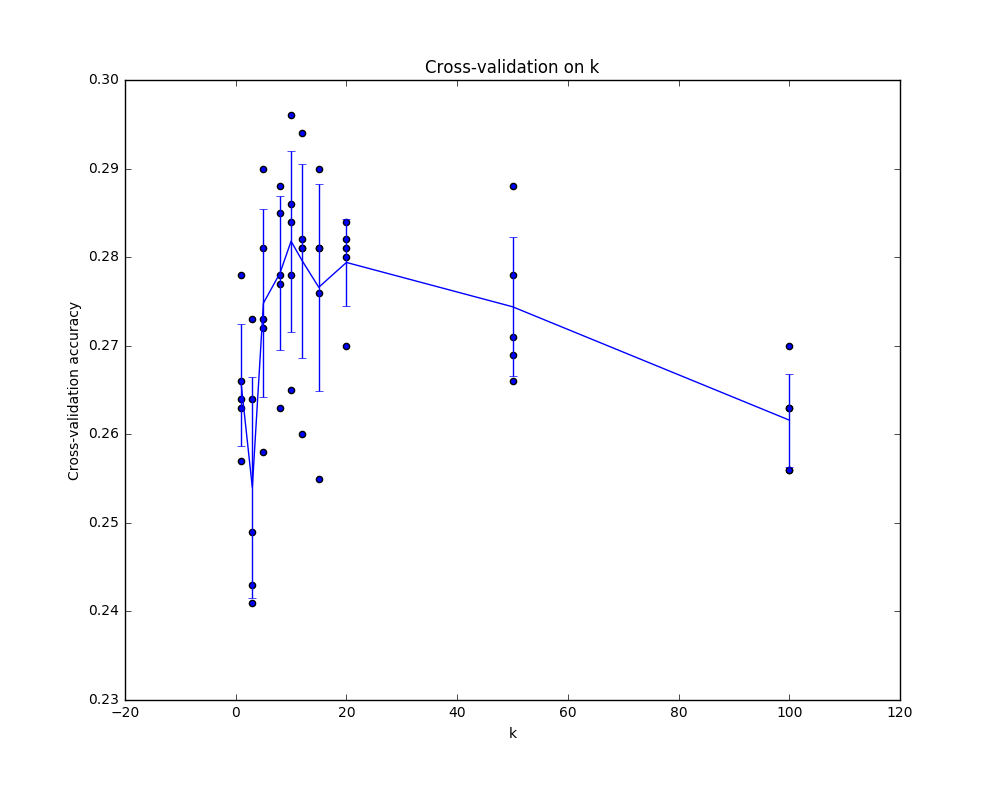
\includegraphics[scale=0.5]{fig1.png}
\end{figure}
We think the best k is $k=3$ and we get $accuracy=139 / 500=0.278000$

\section{Implementing logistic regression}
\subsection{Visualizing the dataset}

\begin{figure}[H]
  \caption{The training data}
  \centering
    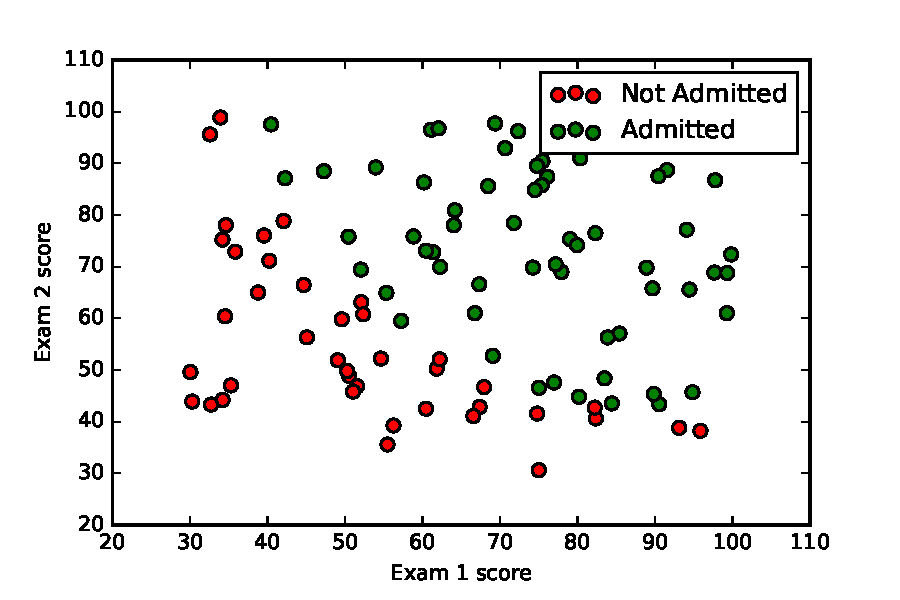
\includegraphics[scale=0.5]{fig1.pdf}
\end{figure}

\subsection{3A1. Implementing logistic regression the sigmoid funciton}
Yes we had tested sigmoid function, it is correct.
\subsection{3A2 Cost function and gradient of logistic regression}
Loss on all-zeros theta vector (should be around 0.693) =  0.69314718056\\
Gradient of loss wrt all-zeros theta vector (should be around [-0.1, -12.01, -11.26]) =  [ -0.1        -12.00921659 -11.26284221]\\
Optimization terminated successfully.\\
         Current function value: 0.203498\\
         Iterations: 19\\
         Function evaluations: 20\\
         Gradient evaluations: 20\\
Theta found by fmin\_bfgs:  $[-25.16056945   0.20622963   0.20146073]$\\
Final loss =  0.203497702351\\

\subsection{Learning parameters using fmin\_bfgs}
\begin{figure}[H]
  \caption{The decision boundary}
  \centering
    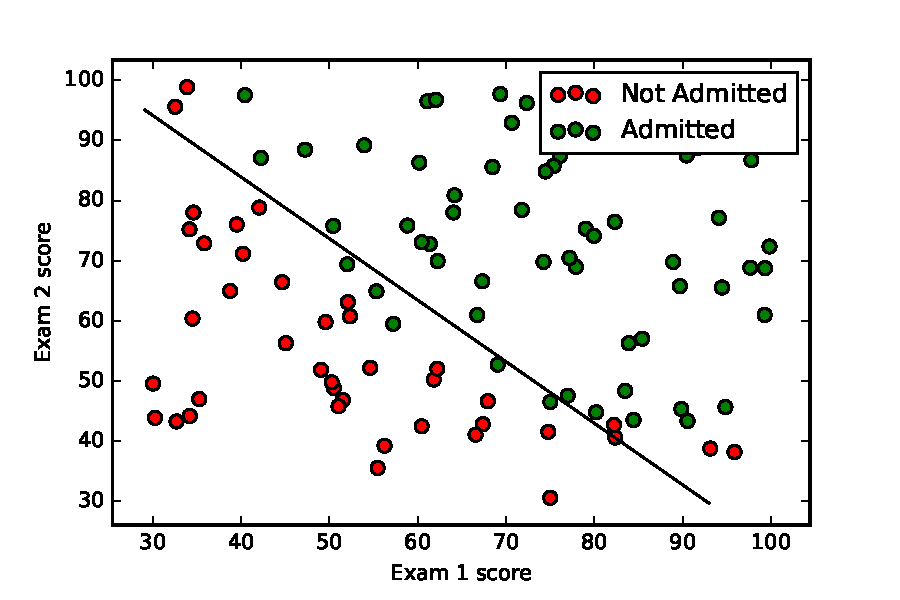
\includegraphics[scale=0.5]{fig2.pdf}
\end{figure}
\begin{figure}[H]
  \caption{The decision boundary from sklearn}
  \centering
    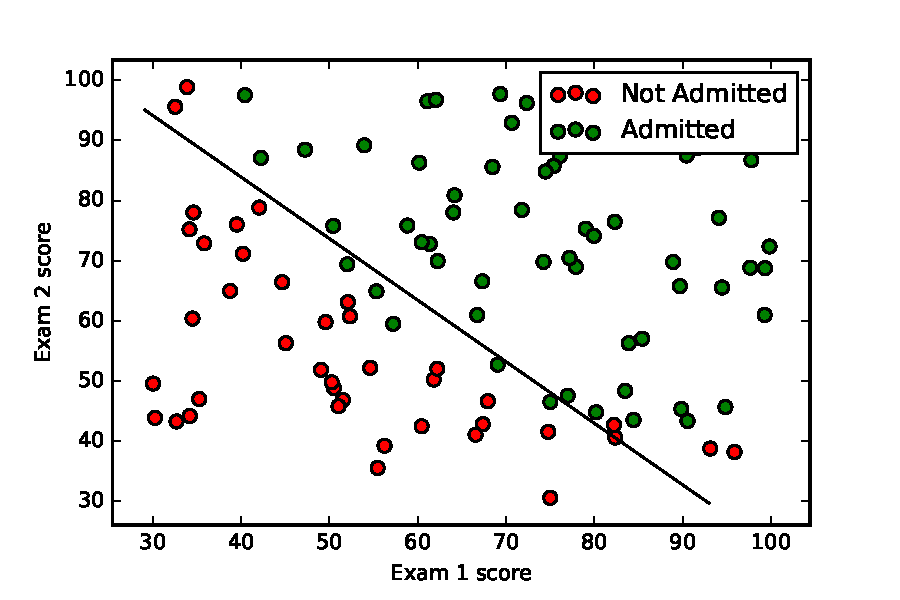
\includegraphics[scale=0.5]{fig2sk.pdf}
\end{figure}
Theta found by sklearn:  [[-25.15293066   0.20616459   0.20140349]]
\subsection{3A3 Prediction using a logistic regression model}
The student with 45/85 score will be admitted with a probability of 0.776246678481.\\
The accuracy on the training set is 0.89.\\

\section{3part B Regularized logistic regression}
\subsection{visualizing the data}

\begin{figure}[H]
  \caption{Plot of training data}
  \centering
    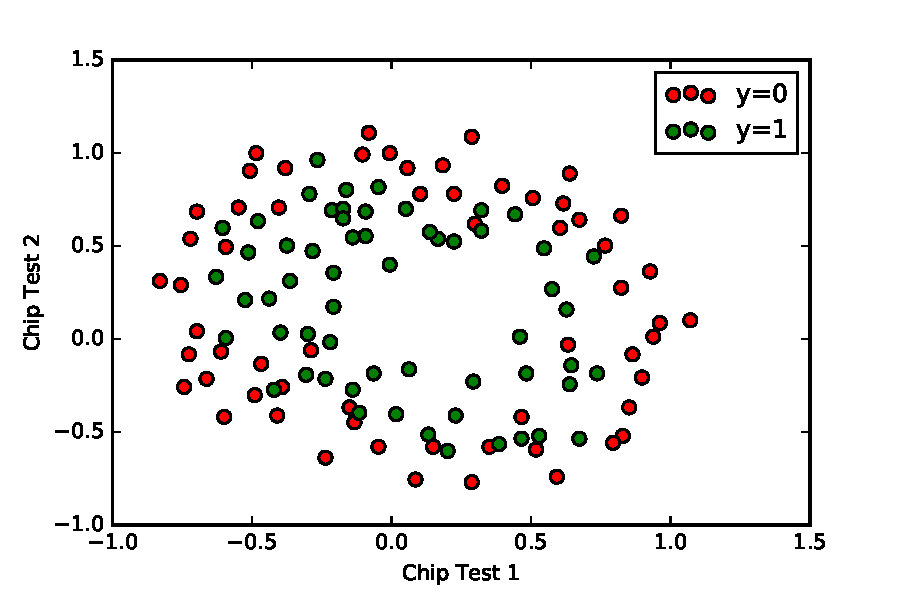
\includegraphics[scale=0.5]{fig3.pdf}
\end{figure}
\subsection{3B1 Cost function and gradient for regularized logistic }

Accuracy on the training set =  0.830508474576
\begin{figure}[H]
  \caption{Traning data with decision boundary for lambda=1}
  \centering
    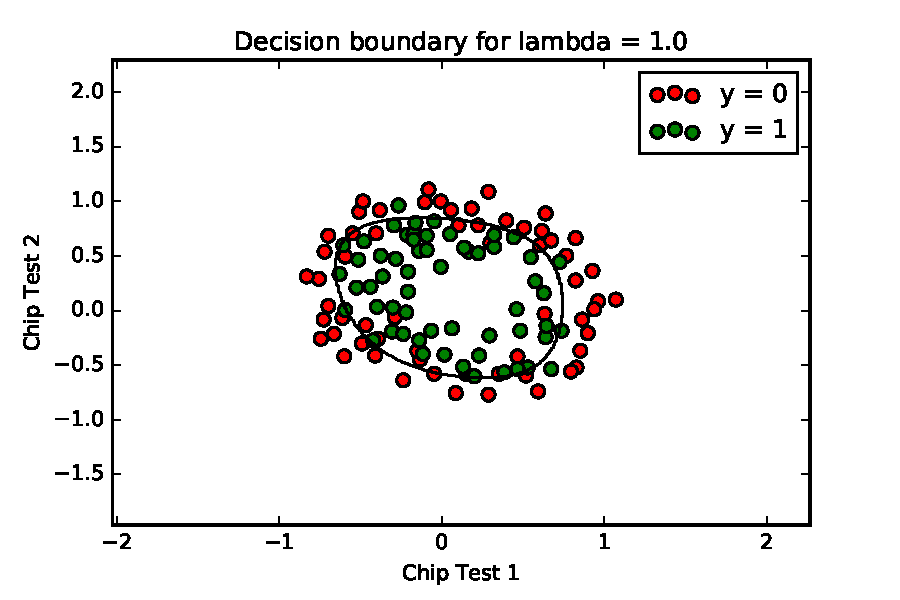
\includegraphics[scale=0.5]{fig4.pdf}
\end{figure}


\subsection{3B2 prediction using the model}

Accuracy on the training set =  0.830508474576





\subsection{3B3 varing lambda}
\begin{figure}[H]
  \caption{lambda=0.1}
  \centering
    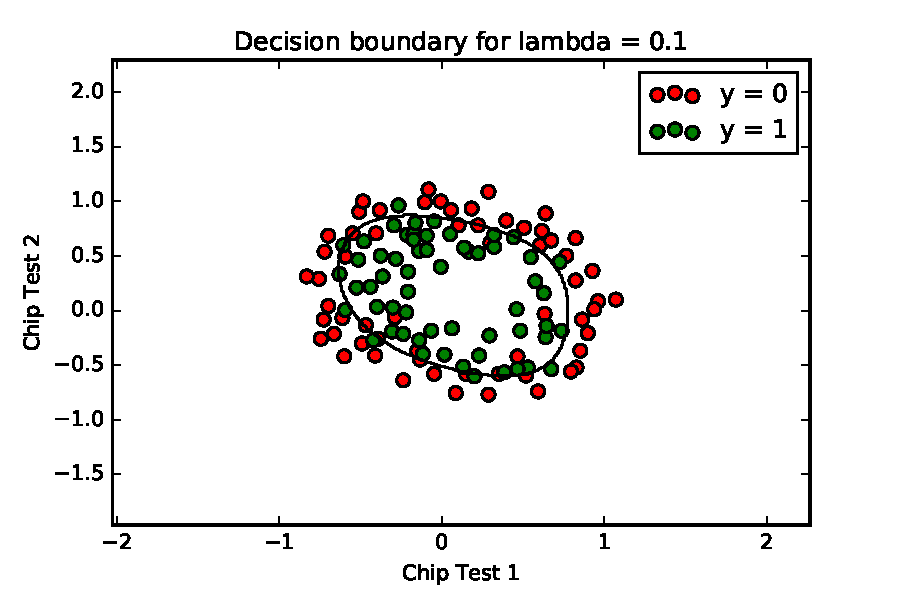
\includegraphics[scale=0.5]{fig401.pdf}
\end{figure}
\begin{figure}[H]
  \caption{lambda=100}
  \centering
    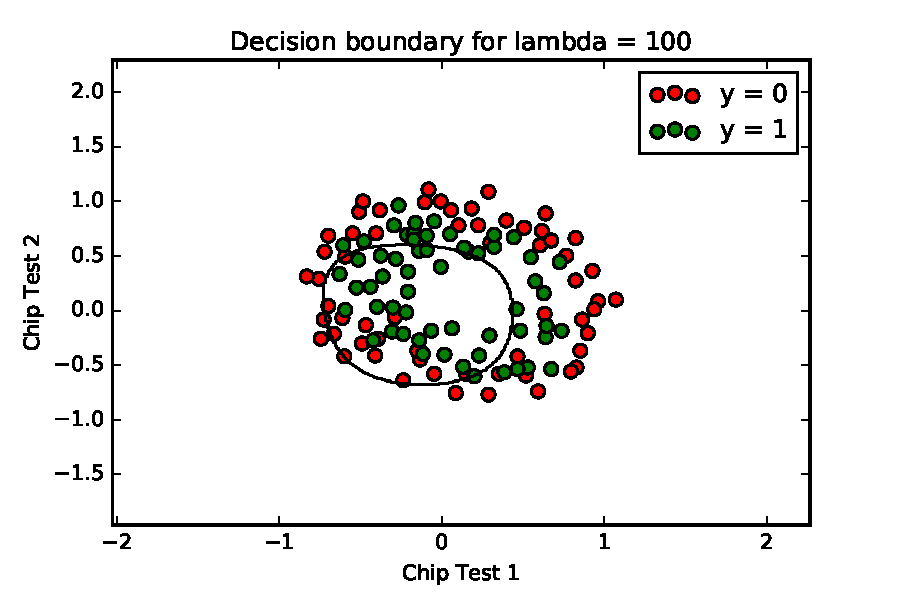
\includegraphics[scale=0.5]{fig4100.pdf}
\end{figure}

\subsection{3B4 Exploring L1 and L2 penalized logistic regression}
\begin{figure}[H]
  \caption{L1sklearn with reg=1}
  \centering
    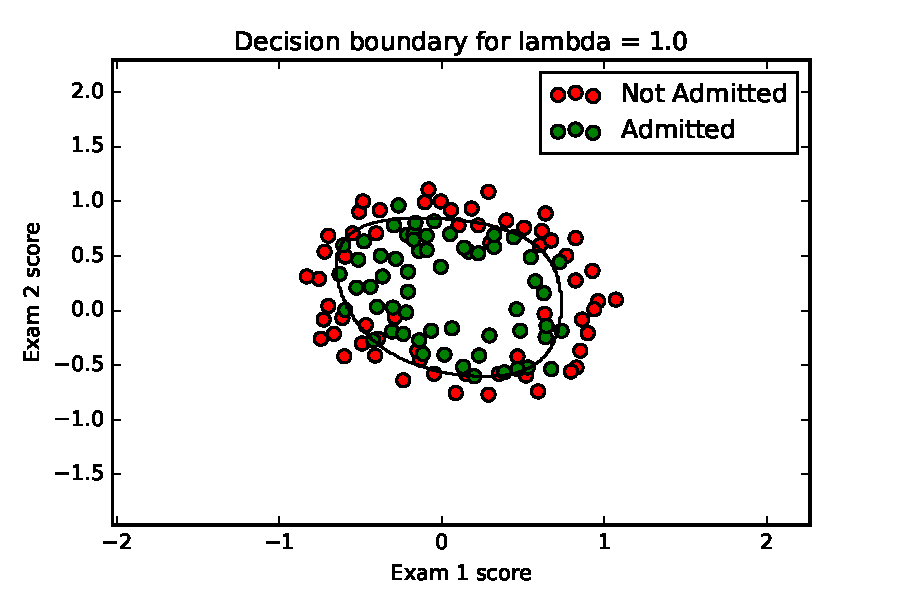
\includegraphics[scale=0.5]{fig4sk.pdf}
\end{figure}
\begin{figure}[H]
  \caption{L1sklearn with reg=0.1}
  \centering
    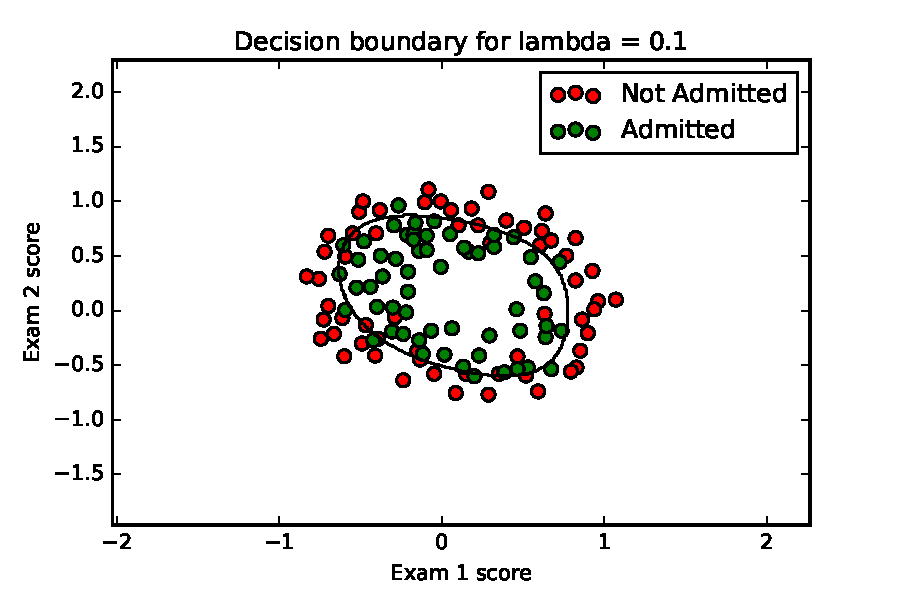
\includegraphics[scale=0.5]{fig4sk01.pdf}
\end{figure}
\begin{figure}[H]
  \caption{L1sklearn with reg=100}
  \centering
    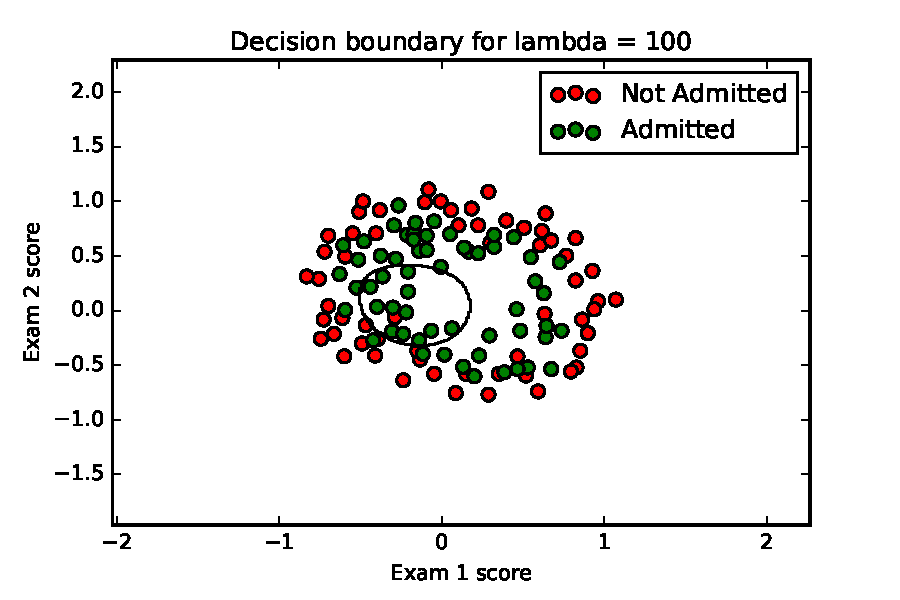
\includegraphics[scale=0.5]{fig4sk100.pdf}
\end{figure}

\subsubsection{with reg=100}
L2sklearn\\
Theta found by sklearn with L2 reg:  [ 0.00468635 -0.01726848  0.0064196  -0.05402665 -0.01327551 -0.03727145
 -0.01821195 -0.00761037 -0.00885306 -0.02224573 -0.04288369 -0.00238585
 -0.01393196 -0.00354828 -0.04072376 -0.02078577 -0.00467203 -0.00354978
 -0.00624894 -0.00500393 -0.03153159 -0.03381515 -0.00108319 -0.00694192
 -0.0003945  -0.00788595 -0.00157683 -0.04058858]
Loss with sklearn theta:  0.68061702032\\
L1\\
Theta found by sklearn with L1 reg:  [ 0.  0.  0.  0.  0.  0.  0.  0.  0.  0.  0.  0.  0.  0.  0.  0.  0.  0.
  0.  0.  0.  0.  0.  0.  0.  0.  0.  0.]\\
Loss with sklearn theta:  0.69314718056
\begin{figure}[H]
  \caption{path}
  \centering
    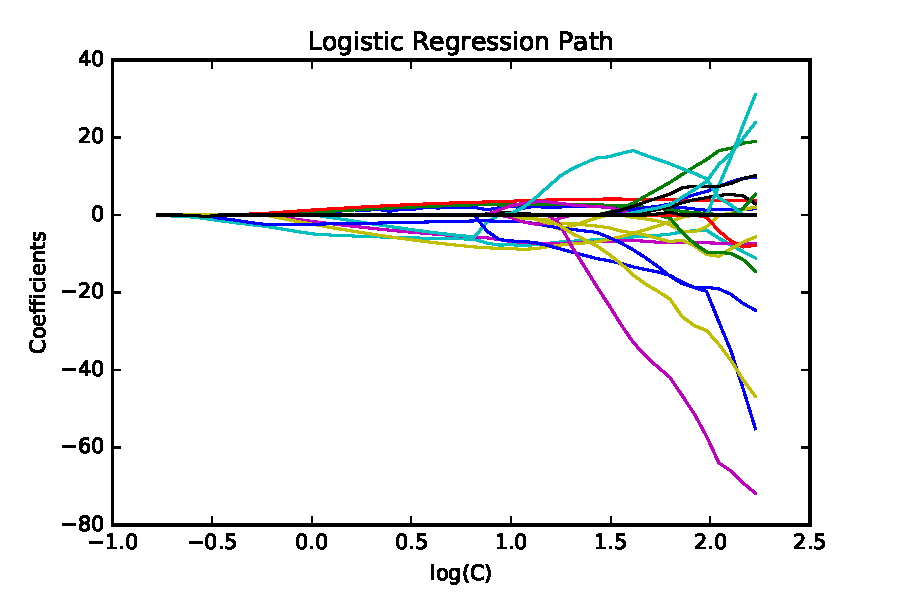
\includegraphics[scale=0.5]{fig5reg100.pdf}
\end{figure}


\subsubsection{with reg=1}
L2sklearn\\
Theta found by sklearn with L2 reg:  [ 1.1421394   0.60141117  1.16712554 -1.87160974 -0.91574144 -1.26966693
  0.12658629 -0.3686536  -0.34511687 -0.17368655 -1.42387465 -0.04870064
 -0.60646669 -0.26935562 -1.16303832 -0.24327026 -0.20702143 -0.04326335
 -0.28028058 -0.286921   -0.46908732 -1.03633961  0.02914775 -0.29263743
  0.01728096 -0.32898422 -0.13801971 -0.93196832]\\
Loss with sklearn theta:  0.46843403006\\

L1sklearn\\
Theta found by sklearn with L1 reg:  [ 1.86965269  0.68661649  1.28041683 -4.86256834 -1.6218069  -2.34227548
  0.          0.          0.          0.          0.          0.          0.
  0.         -2.36743001  0.          0.          0.          0.          0.
  0.          0.          0.          0.          0.          0.          0.
  0.        ]\\
Loss with sklearn theta:  0.438146984954\\
\begin{figure}[H]
  \caption{path}
  \centering
    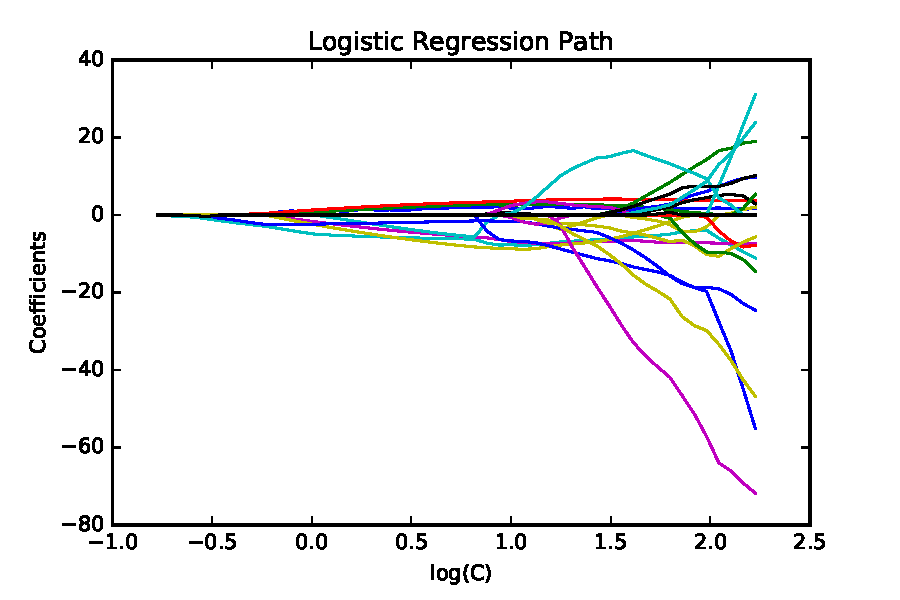
\includegraphics[scale=0.5]{fig5reg1.pdf}
\end{figure}


\subsubsection{with reg=0.1}
L2sklearn\\
Theta found by sklearn with L2 reg:  [ 2.65855183  1.76427994  2.91364412 -4.03385629 -3.34849756 -4.0181188
  0.76777199 -1.08648166 -0.47195071 -0.4774888  -3.27598952  0.54686285
 -1.80180787 -1.17932445 -2.79104067 -0.62127841 -0.4711418   0.61454641
 -1.14697992 -1.20796935 -0.10569617 -2.66246949  0.45857402 -0.76144039
  0.43744164 -1.17502213 -0.93753591 -1.20049576]
Loss with sklearn theta:  0.353830932899\\
L1\\
Theta found by sklearn with L1 reg:  [ 4.00273583  2.56793635  3.56332248 -7.68544357 -6.81244292 -8.6654482
  0.59001851 -0.20079995  0.          0.          0.          2.44529584
  0.          0.         -1.70280933  0.          0.          0.36834145
 -0.66643549  0.          0.         -6.7197063   0.          0.          0.
  0.         -0.05987662  0.        ]\\
Loss with sklearn theta:  0.336434280508\\
\begin{figure}[H]
  \caption{path}
  \centering
    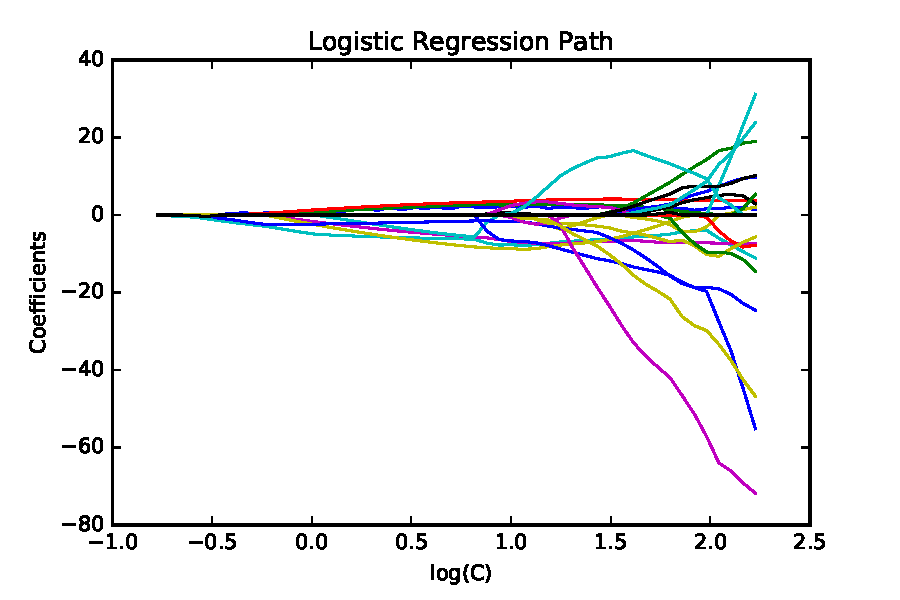
\includegraphics[scale=0.5]{fig5reg01.pdf}
\end{figure}






\subsection{ADSA}






\section{3PART C Logistic regression for spam classification}
best\_lambda =  0.1
Coefficients =  [-4.86311352] [[ -2.74146099e-02  -2.25297669e-01   1.21840891e-01   2.29362945e+00
    2.70425725e-01   2.32851140e-01   9.28595397e-01   2.95200209e-01
    1.62205927e-01   6.78259308e-02  -8.32603904e-02  -1.60373349e-01
   -4.72247939e-02   1.07676991e-02   1.87903695e-01   8.19771795e-01
    5.09529020e-01   3.98710975e-02   2.67729674e-01   3.47047342e-01
    2.60498933e-01   3.64605628e-01   7.25019798e-01   1.96728233e-01
   -3.15395709e+00  -4.03133841e-01  -1.25451038e+01  -6.16577226e-02
   -1.56114586e+00  -5.51430615e-02  -3.00821906e-02   4.07263767e-01
   -3.68156508e-01  -1.43611895e+00  -5.87181904e-01   4.44294672e-01
    4.23159741e-02  -1.56897099e-01  -4.55330705e-01  -1.02250227e-01
   -3.54273314e+00  -1.72944439e+00  -4.37529465e-01  -1.05999940e+00
   -9.18599267e-01  -1.75490296e+00  -1.67475819e-01  -9.56875669e-01
   -3.65653393e-01  -1.36535580e-01  -6.58692608e-02   2.06714067e-01
    1.70694409e+00   1.21460293e+00  -3.35270257e-01   1.56141546e+00
    3.68775545e-01]]
Accuracy on set aside test set for  std  =  0.9296875\\
best\_lambda =  3.1
Coefficients =  [-1.17912402] [[-0.12991085 -0.06968104 -0.10558838  0.52587823  0.44887757  0.21782827
   0.93500336  0.4609256   0.07902944  0.12984314 -0.07793034 -0.19376231
  -0.26408805  0.21343107  0.33108054  0.52441744  0.50983944 -0.05237365
   0.10009654  0.2388837   0.20842673  0.19204128  0.59339178  0.5559746
  -1.15491986 -0.03908939 -1.80938159  0.24677894 -0.16826334  0.04530989
   0.08539098  0.33076073 -0.14508647  0.39233732 -0.26798296  0.44440001
  -0.38065848  0.20745146 -0.25517108 -0.06842383 -0.2217046  -0.7399885
  -0.41435146 -0.5479645  -0.39179324 -0.84827053  0.1179503  -0.47827342
  -0.28401847 -0.09212386  0.02501461  0.76297585  1.30660819  0.06463997
   0.54064182  0.15463283  0.2445029 ]]
Accuracy on set aside test set for  logt  =  0.943359375\\
best\_lambda =  1.1
Coefficients =  [-1.83742964] [[ -1.91463198e-01  -1.66872958e-01  -3.93802023e-01   2.39462779e-01
    9.83292893e-01   1.75311415e-01   2.12183419e+00   7.92547596e-01
    1.94566579e-01   3.34388296e-01  -2.90824615e-01  -4.20297341e-01
   -9.06380382e-01   2.56299856e-01   5.15189474e-01   1.47014136e+00
    8.76696476e-01  -8.32760955e-02   2.41264180e-01   5.01801273e-01
    7.37046896e-01   1.15518007e+00   9.11195183e-01   1.36902984e+00
   -2.35248856e+00  -4.17190307e-01  -3.79772643e+00   6.88337611e-01
   -6.07237597e-01  -1.61622832e-01  -9.24671805e-01  -6.04558747e-01
   -6.91161481e-01  -3.85638234e-02  -6.71440136e-01   3.52732370e-01
   -1.05408408e+00   5.28551480e-01  -7.65306731e-01  -2.46067578e-01
   -1.27643951e+00  -1.90613122e+00  -7.90184279e-01  -1.57619158e+00
   -7.64312034e-01  -2.22366816e+00  -8.34144233e-02  -1.39371572e+00
   -3.06993897e-01   2.00231957e-01  -1.70968577e-01   1.20762876e+00
    1.45771409e+00   3.79908688e-02   5.31812496e-04   5.31812496e-04
    5.31812496e-04]]
Accuracy on set aside test set for  bin  =  0.927734375\\
L1 Penalty experiments -----------\\
best\_lambda =  4.6
Coefficients =  [-1.58224216] [[-0.01058503 -0.15857751  0.12271464  0.20869135  0.24908785  0.17684947
   0.91094465  0.28989815  0.13950775  0.04856944 -0.02293431 -0.13974955
  -0.00711627  0.00919501  0.15436573  0.757055    0.46007631  0.07052224
   0.25407059  0.19614175  0.24321052  0.34684653  0.72790287  0.23451775
  -2.3331197  -0.35827816 -3.14300242 -0.0103872  -0.36948437  0.          0.
   0.         -0.32737303  0.         -0.06123352  0.24264532  0.
  -0.11598013 -0.31175415 -0.04397014 -0.23823111 -0.7937373  -0.19025554
  -0.56287489 -0.73330006 -1.17847525 -0.08550069 -0.51299528 -0.25654505
  -0.1338545  -0.05677716  0.21847266  1.6486311   0.22202108  0.
   0.64874245  0.33267169]]
Accuracy on set aside test set for  std  =  0.921875\\
best\_lambda =  4.6
Coefficients =  [ 0.] [[-0.03108586  0.         -0.05835304  0.21760068  0.42853242  0.16382636
   0.93861109  0.43637043  0.0336125   0.0900391   0.         -0.18979892
  -0.15577098  0.15502515  0.06883162  0.50995193  0.48502309  0.
   0.0816039   0.13837955  0.20244991  0.13150549  0.54632926  0.5352946
  -1.10082093  0.         -1.59018906  0.04169881  0.          0.          0.
   0.         -0.05629357  0.          0.          0.33479349 -0.36265917
   0.         -0.12830472  0.          0.         -0.57434741 -0.00365362
  -0.37647816 -0.34436212 -0.78698577  0.         -0.26116471 -0.04903249
   0.          0.          0.75819977  1.31662069  0.          0.57493288
   0.14286286  0.17451294]]
Accuracy on set aside test set for  logt  =  0.942057291667\\
best\_lambda =  3.6
Coefficients =  [-0.068639] [[ 0.          0.         -0.19387012  0.          0.86592869  0.
   2.02953572  0.63324567  0.02660517  0.21226479  0.         -0.42141844
  -0.68106071  0.          0.          1.31594229  0.76616653  0.
   0.10943515  0.12277559  0.63397775  0.73093098  0.62123301  1.18394328
  -2.42300146 -0.12667642 -3.73091531  0.          0.          0.          0.
   0.         -0.28838226  0.         -0.21913877  0.         -1.01538095
   0.         -0.40473594  0.         -0.11526309 -1.69430107 -0.03936989
  -1.11032049 -0.68712656 -2.21929271  0.         -1.02593714 -0.1251873
   0.07427587  0.          1.14962067  1.49992422  0.         -0.6282075
  -0.76757788 -0.20228585]]
Accuracy on set aside test set for  bin  =  0.92578125










\section{Implementing logistic regression}
\subsection{Logistic regression}
\begin{itemize}
\item Cost with zero vector: 0.69314718056
\item Gradient with zero vector: $[ -0.1,        -12.00921659, -11.26284221]^T$
\item Cost with {\tt fmin\_bfgs}: 0.203497702351
\item Accuracy: 0.89

\end{itemize}

\subsection{Regularized logistic regression}
\begin{itemize}
\item Accuracy: 0.830508474576

\item As expected, L1 regularizes most coefficients to go to 0, while L2 forces coefficients to be small but remain nonzero. Increasing $\lambda$ forces more (eventually all) coefficients to zero in L1 and even smaller coefficients in L2, while decreasing does the opposite.
\item The loss continues to increase with the regularization parameter, until $\theta$ approximates the zero vector, in which case the loss plateaus.
\item With lower thetas, we found that L1 regularization performs better. However as we increase thetas above 1, we see found that L2 regularization was superior. Because loss increased as we increased lambda, the best loss values occurred with lower lambda values, meaning L1 regularization proved superior in this case. 
\end{itemize}

\subsection{Logistic regression for spam classification}
\begin{table}[h]
\caption{Best $\lambda$ and accuracy for different feature transforms}
\centering
\begin{tabular}{r || c c | c c}
& L1 $\lambda$ & L1 Accuracy & L2 $\lambda$ & L2 Accuracy\\
\hline
STD & 4.6 & 0.9219 & 0.1 & 0.9297\\
LOGT & 4.6 & 0.9421 & 4.6 & 0.9434\\
BIN & 3.6 & 0.9258 & 1.1 & 0.9277\\
\end{tabular}
\end{table}
As expected, the model sparsity is greater for L1 than for L2. This is because L1 regularization forces coefficients to go to zero more often. We suggest using L1 with the log transform. The log transform seems to yield the highest accuracy in both regularization techniques, but L1 forces many of the feature coefficients to zero, making the model easier to interpret. We can get rid of features that are irrelevant and lower the chance of overfitting.

\pagebreak
\subsection{Classifying music genres}
\begin{itemize}
\item We tried running the classifier with various regularization parameters, from $\lambda=0.1$ to $\lambda=10000$. We found that the best accuracy occurs around $\lambda=30$, using the Mel Cepstral representation and L1 regularization. This gave us $50-55\%$ accuracy. Even after varying lambdas, Mel Cepstral with L2 regularization and both FTT models gave around $30\%$ accuracy.
\item Classical music is the easiest genre to classify. We are able to correctly identify $>90\%$ of classical pieces.
\item Metal music is a difficult genre to classify. Although our classifier correctly classifies most metal pieces correctly as metal, metal unfortunately confuses our classifier and causes it to classify most pieces as metal music as well, especially for the Mel Cepstral representation. On the other hand, rock has the highest classification error, which means our classifier fails to identify rock correctly.
\item To improve the accuracy of the one vs. all classifier, you could require that the maximum value given by our maxarg have a threshold of confidence above the next couple lowest values. If the likelihood that our example $x$ belongs to class $k$ is within the threshold, we rerun the OVA model with all $k$ that meet the threshold within the max.  
\item Use of a Softmax OVA as given in section 2.1 of the following paper could also lead to some potential improvements: \url{http://www.gatsby.ucl.ac.uk/~chuwei/paper/smc.pdf}
\end{itemize}

\pagebreak
\section*{Appendix}
\begin{figure}[H]
  \caption{Scores of students vs. Admittance}
  \centering
    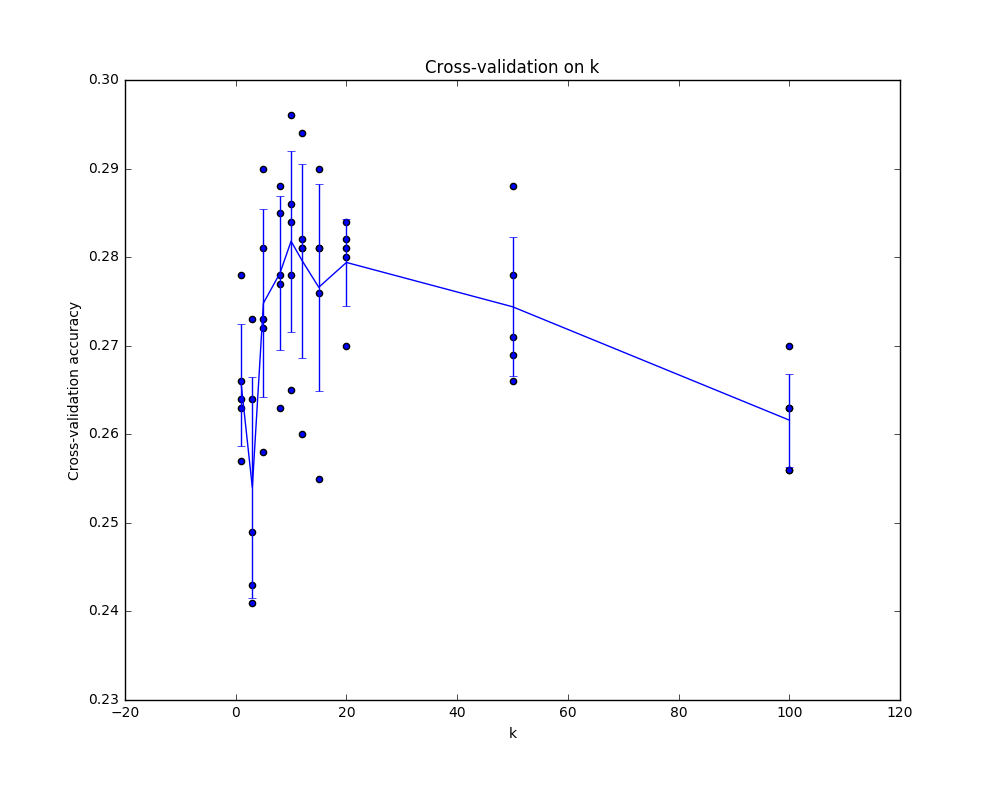
\includegraphics[scale=0.5]{fig1.png}
\end{figure}
\begin{figure}[H]
  \caption{Decision boundary}
  \label{fig:linfit}
  \centering
    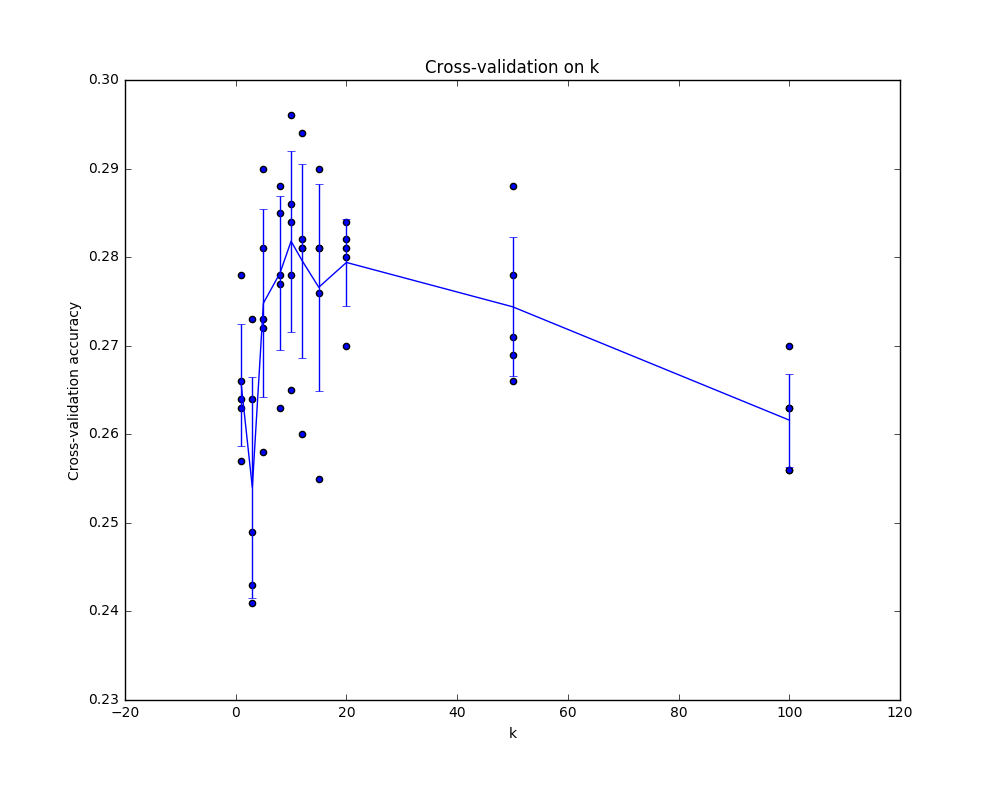
\includegraphics[scale=0.5]{fig1.png}
\end{figure}






\end{document}